\section{Workshop outline}
\label{sec:intro}
\tikzsetexternalprefix{./introduction/tikz/}

\subsection{Goals}
    \paragraph{}
    The main goal of this workshop is to give you a brief overview of what a standard \gls{acr:md} workflow would look like. We shall be covering some of the core techniques used to set up and run a variety of different calculations including \textbf{molecular docking}, \textbf{molecular dynamics} and \textbf{free energy} calculations. We shall also briefly cover some analysis techniques available and some other resources available to further your understanding of the techniques used throughout. 

    \paragraph{}
    The steps of the workshop are as follows:
    \begin{itemize}
        \item Locate and download the crystal structure
        \item Dock the ligand into the active site
        \item Parameterise the ligand
        \item Create molecular dynamics input files
        \item Run a simple dynamics simulation
        \item Perform simple trajectory analysis
        \item Calculate the binding energy of the ligand
    \end{itemize}

\begin{figure}[H]
    \centering
    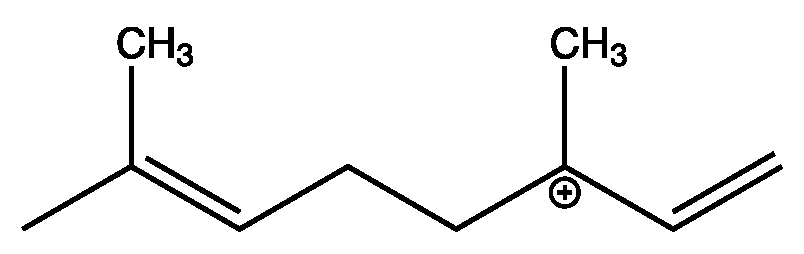
\includegraphics[width=0.7\textwidth]{Graphics/1n20Lig.eps}
    \caption{Ligand used within the workshop.}
    \label{fig:Lig}
\end{figure}

    \paragraph{}
    We shall be using a ligand (\cref{fig:Lig}) from a study by Major et. al.\cite{Weitman2010ChallengesMonoterpenes} due to personal experience working with Terpene synthesis. For more information about the system, please see the previous work. 

\subsection{Software}
    \paragraph{}
    The key software that we will be using for this workshop is all free to use and should be simple to access and use. Most of the software however requires a basic understanding of how to use the \gls{acr:cli}. It is possible to use all of the software from within Windows but Linux is recommended for the smoothest experience. The \enquote{Cheat Codes} in \cref{sec:Cheats} at the end of this document has only been tested in a pure Linux \gls{acr:os}.

    \paragraph{}
    The required software for this workshop is as follows:
\begin{itemize}
    \item \href{https://www.anaconda.com/download/}{anaconda}
    \item \href{https://learn.microsoft.com/en-us/windows/wsl/install}{WSL2} (windows only)
    \item \href{https://ambermd.org/GetAmber.php}{AMBER}\cite{Maier2015Ff14SB:Ff99SB} \footnote{It is recommended that you install the full (paid) version of amber for production dynamics due to the GPU support, however for individual machines and the purpose of this workshop, the conda binary distribution is okay.}
    \item \href{https://www.ks.uiuc.edu/Development/Download/download.cgi?PackageName=VMD}{VMD}\cite{WilliamHumphrey1996VMDDynamics}
    \item \href{https://github.com/gnina/gnina}{gnina}\cite{McNutt2021GNINALearning}
    \item \href{https://pypi.org/project/acpype/}{acpype} \cite{SousadaSilva2012ACPYPEInterfacE} \footnote{A web server version of acpype is available \href{https://www.bio2byte.be/acpype/submit/}{here} for users unable to install, however installing this is highly recommended where possible.}
\end{itemize}

    \paragraph{}
    Although not required for this workshop, some other software that is available to assist with the \gls{acr:md} workflow are as follows:

\begin{itemize}
    \item CHARMM\cite{Brooks1983CHARMM:Calculations} (\gls{acr:md} package)
    \item gromacs\cite{Berendsen1995GROMACS:Implementation} (Open source \gls{acr:md} package)
    \item CGenFF\cite{Vanommeslaeghe2012AutomationTyping} (Forcefield parameterisation tool for the CHARMM forcefield)
    \item pyMol (\gls{acr:gui} for molecular visualisation and manipulation)
    \item AutoDock4\cite{Morris2009AutoDock4Flexibility} (Open source docking software)
    \item YASARA\cite{Krieger2014YASARAWorkstations} (\gls{acr:gui} for the whole \gls{acr:md} workflow)
    \item Alphafold\cite{Jumper2021HighlyAlphaFold, Varadi2022AlphaFoldModels} (Open source A.I. homology modelling software) 
\end{itemize}


